\documentclass[stu,12pt]{apa7}
\usepackage{graphicx}
\usepackage{amsmath}
\usepackage{tabularray}
\usepackage{siunitx}
\UseTblrLibrary{siunitx}
\usepackage{float}
\usepackage[american]{babel}
\usepackage{csquotes}

\usepackage[style=apa, backend=biber]{biblatex}
\addbibresource{bibliography.bib}

\title{Redistribution Policies and Consequences for Civil Unrest: The Case of the \textit{Bolsa Família} Conditional Cash Transfers in Brazil}
\author{Júlia Quintaneiro Pimenta}
\shorttitle{}
\affiliation{\mbox{Master in the Social Sciences, Universidad Carlos III de Madrid}}
\course{19307: Political Economy}
\professor{Işık Özel, Sebastián Lavezzolo, Dulce Manzano}
\duedate{19 June 2026}

\abstract{
Cash transfer programmes have been shown to have not only favourable effects in relieving poorer families from financial burdens, but also lead to spillovers in unintended areas. Particularly, evidence may suggest that with an increase in cash transfers, personal and collective violence decreases. In this paper, the impact of Brazil’s \textit{Bolsa Família} programme on violent unrest was explored. In particular, the moderating effect of relative deprivation, which is believed to dampen the benefits of the cash transfers, was investigated as a potential mechanism, as it has been unexplored for this association to date. The interaction was tested using a two-way fixed effects Linear Probability Model with municipal-level binary violent counts as an outcome. Results show that there is a negative and significant correlation between payments and violence in Brazil. Additionally, the interaction effect is positive and significant, which supports the expectation that relatively deprived municipalities will experience a lesser negative effect, meaning that cash transfers have less impact on reducing violent unrest. However, concerns with a low within R\textsuperscript{2} are flagged as a major limitation, as it may indicate that the fixed effects drive most of the association. The results and their implications are discussed.
}
\keywords{conditional cash transfers, Brazil, civil unrest, violence, relative deprivation}

\begin{document}

\maketitle

Among the most successful redistribution programmes, Brazil’s \textit{Bolsa Família}—or Family Allowance—stands out, with documented success at eradicating poverty among the Brazilian population and being copied by other countries \parencite{franConditionalCashTransfers}. \textit{Conditional cash transfer} (CCT) programmes are, most generally speaking, programmes that “transfer cash, generally to poor households, on the condition that those households make prespecified investments in the human capital of their children” \parencite[1]{franConditionalCashTransfers}. In other words, by complying with certain conditions, a household could be eligible to receive benefits that alleviate financial burdens. The \textit{Bolsa Família} was introduced in 2003 by the then-president Luiz Inácio Lula da Silva, who consolidated different programmes and created a unified registry, which facilitated bureaucratic hurdles and created the largest CCT programme at that time \parencite{PDFNutsBolts}. Families were considered eligible if they earned less than a certain amount of money, their children attended school, and were up-to-date on vaccines, among other things \parencite{PDFNutsBolts}.

When Jair Bolsonaro took office in 2019, he reformed the programme, which was rebranded as \textit{Auxílio Brasil}. The new programme was restructured to be expanded to more families, but also experienced criticism for funding uncertainty \parencite{figueiredoProgramaAuxilioBrasil2022}. When Lula took Bolsonaro’s position, he reintroduced the \textit{Bolsa Família} programme as \textit{Novo Bolsa Família} \parencite{valeEfeitoAumentoNo2025a}. Therefore, the programme has experienced large restructuring over the last years.

Beyond its beginnings, the success of the programme has been documented. By following children for over a decade, it has been found that receiving the CCTs led to significantly better socioeconomic conditions \parencite{fassarellaSocialMobilityCCT2024}. In the data, 64\% of the people who received benefits were no longer beneficiaries, and 45\% of beneficiaries accessed the formal labour market. This evidence shows that receiving CCTs from the \textit{Bolsa Família} programme increases social mobility and thus improves the lives of current and former beneficiaries at an individual level \parencite{fassarellaSocialMobilityCCT2024}.

While the individual-level effects of the CCTs have been documented, potential spillovers to unintended areas have been in debate \parencite{gerardCashTransfersFormal2021}. Particularly in terms of societal-level implications, the consequences on violence have been discussed, with CCTs being tied to a reduction in crime in urban Brazil as well as murder rates for both Brazil and Mexico \parencite{chiodaSpilloversConditionalCash2016, lanceConditionalCashTransfers2014}. The link between payments and violence and what mechanisms influence it is thus not only of academic, but also societal relevance. Understanding spillovers might help assess consequences of CCTs which might be, at first, unintentional, but potentially beneficial.

To address this theoretical question, it will be investigated in this paper how redistributive policy, more specifically the CCT programme \textit{Bolsa Família} in Brazil—which will hereafter encompass all its versions until now—, impacts the occurrence of violent unrest in the country. As such, the question that will be addressed is thus the following: To what extent are municipal-level \textit{Bolsa Família} CCTs associated with lower violent unrest in Brazil, and do varying levels of relative deprivation moderate the relationship?

The paper will be structured as follows: First, the current state of the literature will be discussed, which will lead to the development of a theoretical framework explaining the proposed mechanism and the hypotheses. Secondly, the method will be elaborated, and the results of the analysis presented. Finally, the results will be discussed in light of the literature.

\section{Theoretical Background}

\subsection{Spillover Effects of Conditional Cash Transfers}

Previously, the topic was introduced and the research question established. In this section, literature tied to the potential spillover effects of CCTs will be reviewed. In general, CCT programmes have been found to have unintended secondary effects. While they are mainly meant to reduce poverty, the programmes have produced spillovers in a variety of other areas. In Brazil, \textcite{machadoConditionalCashTransfer2018} investigated whether the \textit{Bolsa Famíli}a CCT programme led to a reduction in crimes and hospitalisation from violence. To do that, they used panel data from 2004 to 2012 to run fixed effects regression models. The results showed that as the CCT coverage increased, both crime and hospitalisation rates decreased significantly \parencite{machadoConditionalCashTransfer2018}. This shows that there seems to be an unintended spillover of CCTs on violence—the higher the coverage, the lower the violence.

The connection with crime was further established by \textcite{chiodaSpilloversConditionalCash2016}. They investigated whether an expansion of the \textit{Bolsa Família} programme was tied to a significant reduction in crime in the city of São Paulo. In their research, they found that there was a negative relationship with crime. In other words, as the programme expanded, there was a noticeable reduction in violent crimes, which further emphasises the connection \parencite{chiodaSpilloversConditionalCash2016}.

In terms of violent mobilisation, research in Colombia shows a clear negative effect of CCTs \parencite{penaCivilConflictConditional2017}. Through a difference-in-differences approach, \textcite{penaCivilConflictConditional2017} find that CCT programme rollout impacted the demobilisation of armed combatants. The context is different from the one in Brazil: At that time, Colombia was experiencing internal conflict, and additionally, the armed groups recruited children, who were eligible for the CCT programme after rollout. However, this is to exemplify how CCTs can negatively affect collective violence \parencite{penaCivilConflictConditional2017}. In other words, with an increase in payments, there is an observable decrease in violence.

The link to general reduction of violence has also been shown on the more individual level. This can be exemplified through studies on domestic violence. With an increase in CCT payments, domestic violence significantly decreases \parencite{litwinConditionalCashTransfer2019, borrazConditionalCashTransfers2020}. This decrease in violence both on the individual and collective level could be explained through the reduction of material grievances. As the payments increase, poorer households hold fewer grievances, which in turn decreases violence both individually and collectively. Collectively, it could manifest through a reduction in violent unrest, such as violent crimes, riots, or violent protests.

More recent publications question the previously established link. \textcite{zizumbo-colungaUnintendedConsequencesConditional2023} analysed the link between the introduction of the Mexican CCT programme and violence. The expansion of the programme was associated with an increase in violence in his data \parencite{zizumbo-colungaUnintendedConsequencesConditional2023}. However, given the vast evidence that the link is rather negative, it can—in sum—be said that for the case of Brazil, it can be expected that an increase in payments could be generally related to a decrease in collective violence.

\subsection{Relative Deprivation}

Having established the current literature previously, in this section, the proposed mechanism will be elaborated upon. In general, \textit{Relative Deprivation Theory} theorises that if individuals believe they are relatively more deprived through upward comparison, they might develop grievances and anger \parencite{smithRelativeDeprivationTheory2020}. Relative deprivation is associated with individual deviance, such as crime, but also collective action \parencite{smithRelativeDeprivationTheory2020}. When it is operationalised, it can be proxied through income inequality \parencite{aransiolaEffectAbsoluteRelative2021}.

Previous research has found deprivation to be an important factor influencing violent events in a country. \textcite{aransiolaEffectAbsoluteRelative2021} investigate how deprivation affects homicides in Brazil, namely absolute deprivation, which is proxied through unemployment, and relative deprivation, proxied through income inequality. They find that both have an influence on homicide levels. Additionally, they exacerbate each other \parencite{aransiolaEffectAbsoluteRelative2021}. The same has been observed in other countries. In the United States, absolute and relative deprivation were also found to have a significant interaction in predicting violent crimes \parencite{burrastonRelativeAbsoluteDeprivations2018}. Therefore, it can be concluded that deprivation plays a role in violence: Higher deprivation is associated with higher rates of homicides.

On an individual level, the feeling of being relatively deprived predicts aggression levels. In a longitudinal study, \textcite{greitemeyerImpactPersonalRelative2019} examined whether feelings of relative deprivation predicted later reported aggression. When controlling for earlier aggression levels, deprivation was still a significant predictor of later reported levels \parencite{greitemeyerImpactPersonalRelative2019}. In addition, deprivation has been tested as a potential mechanism in models concerning aggression. In the link between feeling ostracised and personal aggression levels, relative deprivation significantly mediated the relationship \parencite{jiangRelativeDeprivationMechanism2020}.

The individual level also seems to play a role when using violent crimes as an outcome. \textcite{itskovichEconomicInequalityRelative2025} used a Cox Proportional Hazard Model to investigate whether relative deprivation increases the chances of an individual committing a violent crime in the long term. He finds that the chance of committing a violent crime indeed increases. This further confirms the link to aggression established by previous literature \parencite{itskovichEconomicInequalityRelative2025, greitemeyerImpactPersonalRelative2019, jiangRelativeDeprivationMechanism2020}.

Thus, it becomes clear that relative deprivation might help in explaining variation in violent unrest. Although often used as an explanatory mechanism, it has not been applied yet to the CCT–violence link proposed in this paper. As such, testing the mechanism would fill an important gap in current research. This highlights the academic relevance of conducting this research.

\subsection{Hypotheses}

In sum, previous studies have shown that CCTs can have unintended spillover effects. In São Paulo, they were shown to have led to a reduction in crime \parencite{chiodaSpilloversConditionalCash2016}. Additionally, the Colombian CCT programme was associated with a demobilisation of combatants \parencite{penaCivilConflictConditional2017}. In general, there seems to be a negative relationship between CCTs and violence, which is expected to be reflected in the case of violent mobilisation.

Following the theory, CCTs—as a redistributive policy—could reduce material grievances, which could reduce violent mobilisation. Thus, it is hypothesised that municipalities that proportionally received more CCTs show, on average, less violent unrest (H\textsubscript{1}). Additionally, it is hypothesised that the relationship is moderated by relative deprivation, with higher deprivation weakening the suppressive effects of CCTs (H\textsubscript{2}).

\section{Method}

\subsection{Sample and Data}

The sample consists of the 5,293 municipalities of Brazil, with data spanning from January 2018 to March 2026. This gives a total of 557,198 observations in the data (\textit{N} = 557,198). The log-transformed CCT payments value is the main predictor (\textit{M} = 5.75, \textit{SD} = 0.62). The outcome is a binary variable on violent unrest. The moderator is a relative deprivation measure (\textit{M} = -42.74, \textit{SD} = 216.36). Full descriptive statistics can be found in Table 1.

\begin{table}
\caption{Descriptives}
\centering
\begin{tblr}[         %% tabularray outer open
]                     %% tabularray outer close
{                     %% tabularray inner open
colspec={Q[]Q[]Q[]Q[]Q[]Q[]Q[]},
hline{2}={1-7}{solid, black, 0.05em},
hline{1}={1-7}{solid, black, 0.08em},
hline{4}={1-7}{solid, black, 0.08em},
column{1}={}{halign=l},
column{2-7}={}{halign=r},
}                     %% tabularray inner close
& N & Mean & SD & Median & Min & Max \\
CCT Payment & 557006 & \num{5.75} & \num{0.62} & \num{5.51} & \num{4.25} & \num{6.94} \\
Relative Deprivation & 557198 & \num{-42.74} & \num{216.36} & \num{-18.64} & \num{-410.85} & \num{703.06} \\
\end{tblr}
\end{table}


\subsection{Data Cleaning and Preparation}

For the main variables of interest, the data were sourced from three different data sets. The independent variable (IV)—\textit{municipal-level CCTs}—was operationalised through the monthly data on the different CCT programmes as provided by the \textcite{CECAD20a}. \textit{Bolsa Família} data is available for the period from January 2018 to November 2021, \textit{Auxílio Brasil} for the period from November 2021 to February 2023, and \textit{Novo Bolsa Família} for the period from March 2023 to March 2026. For every month, the average CCTs received per municipality were calculated, which will be used as the IV. Note that the final data does not differentiate between the different programmes, i.e., \textit{Bolsa Família}, \textit{Auxílio Brasil}, and \textit{Novo Bolsa Família}. Spatial data as provided by \textcite{pradoKelvinsMunicipiosbrasileiros2026} was merged with the CCT data.

The dependent variable (DV) was sourced from the \textcite{ACLED2026}. \textit{Violent unrest} was operationalised through violent demonstration, mob violence, excessive force against protesters, and protest with intervention from the available sub-event types. Given that data are sparse for violent unrest, especially on the municipal level, a binary variable was created that indicates whether a given municipality experienced a violent event or not. Additionally, the data were selected to coincide with the monthly CCTs, meaning from January 2018 to March 2026.

Relative deprivation, which will act as the moderator, was calculated through the average income \parencite{Tabela7395Rendimento}. As there is no available data on the average income at the municipal level, the average income of each state was used. As relative deprivation represents the perceived deprivation conceptually in contrast with others, it was operationalised by taking the difference between the respective state’s and national average income. Although income differs by year as well, the same amount is used across all months, which was calculated by averaging the available data for the average 2019 to 2024 income.

\subsection{Procedure}

An ordinary least squares (OLS) linear probability model (LPM) with two-way fixed effects will be estimated to analyse the relationship between CCTs and violent unrest in Brazil, using relative deprivation as the interaction term, with the alpha set at .05. The specific fixed effects will be municipality and time fixed effects. Additionally, the model will use clustered standard errors on the municipal level, which accounts for correlations within the same municipality across time. The model will thus be fit as follows:
\[violence_{it} = \beta_0 + \beta_1log(transfer)_{it} + \beta_2(log(transfer)_{it} \times reldepr_i) + \alpha_i + \gamma_t + \varepsilon_{it}\]
The full analysis as well as diagnostics can be found in the supplementary repository \parencite{zotero-item-1650}.

\section{Results}

\subsection{Baseline Model}

An LPM using two-way fixed effects was run to examine the relationship between municipality-level CCTs and violent unrest in Brazil. In the data, the relationship was shown to be negative and significant, \textit{b} = -0.0021, \textit{SE} = 0.0010, \textit{t} = -2.074, \textit{p} = .038. In other words, for every one-per cent increase in CCT payments, there is an expected 0.21\% decrease in violent unrest for a given municipality. However, the results show that the within R\textsuperscript{2} of the model is very low, \textit{R\textsuperscript{2}} = .0000087. This means that the fixed effects might be capturing most of the variation in the violent events, rather than the CCT payments.

\subsection{Interaction Effect}

To test a potential mechanism for the relationship, relative deprivation was added as an interaction term to the main analysis, which investigates the relationship between municipality-level CCTs and violent unrest in Brazil. The interaction term affected the relationship positively and significantly, \textit{b} = 0.0000040, \textit{SE} = 0.0000018, \textit{t} = 2.22, \textit{p} = .026. As such, for each one-unit increase in the relative deprivation measure, the relationship between CCTs and violence increases by 0.00040\%. Thus, in more deprived areas, CCTs are shown to be less effective in reducing the overall violent unrest. Again, the within R\textsuperscript{2} is low, which is an important limitation, \textit{R\textsuperscript{2}} = .000057. It is, however, slightly higher than in the baseline model, which indicates that the interaction term added additional, although negligible, explanatory power. The results for both the baseline and the interaction model can be found in Table 2, and the marginal effects plot can be found in Figure 1.

\begin{table}
\caption{LPM Results}
\centering
\begin{talltblr}[         %% tabularray outer open
entry=none,label=none,
note{}={+ p \num{< 0.1}, * p \num{< 0.05}, ** p \num{< 0.01}, *** p \num{< 0.001}},
]                     %% tabularray outer close
{                     %% tabularray inner open
colspec={Q[]Q[]Q[]},
hline{2}={1-3}{solid, black, 0.05em},
hline{8}={1-3}{solid, black, 0.05em},
hline{1}={1-3}{solid, black, 0.08em},
hline{18}={1-3}{solid, black, 0.08em},
column{2-3}={}{halign=c},
column{1}={}{halign=l},
}                     %% tabularray inner close
& Baseline & Interaction \\
log\_payment & \num{-0.002}* & \num{-0.004}** \\
& (\num{0.001}) & (\num{0.001}) \\
rel\_deprivation &  & \num{-0.000}* \\
&  & (\num{0.000}) \\
log\_payment × rel\_deprivation &  & \num{0.000}* \\
&  & (\num{0.000}) \\
Num.Obs. & \num{557006} & \num{557006} \\
R2 & \num{0.234} & \num{0.234} \\
R2 Adj. & \num{0.227} & \num{0.227} \\
R2 Within & \num{0.000} & \num{0.000} \\
R2 Within Adj. & \num{0.000} & \num{0.000} \\
AIC & \num{-1336668.5} & \num{-1336691.7} \\
BIC & \num{-1276114.5} & \num{-1276115.3} \\
RMSE & \num{0.07} & \num{0.07} \\
FE: muni\_norm & X & X \\
FE: time\_id & X & X \\
\end{talltblr}
\end{table}


\begin{figure}
    \centering
    \caption{Interaction Effect}
    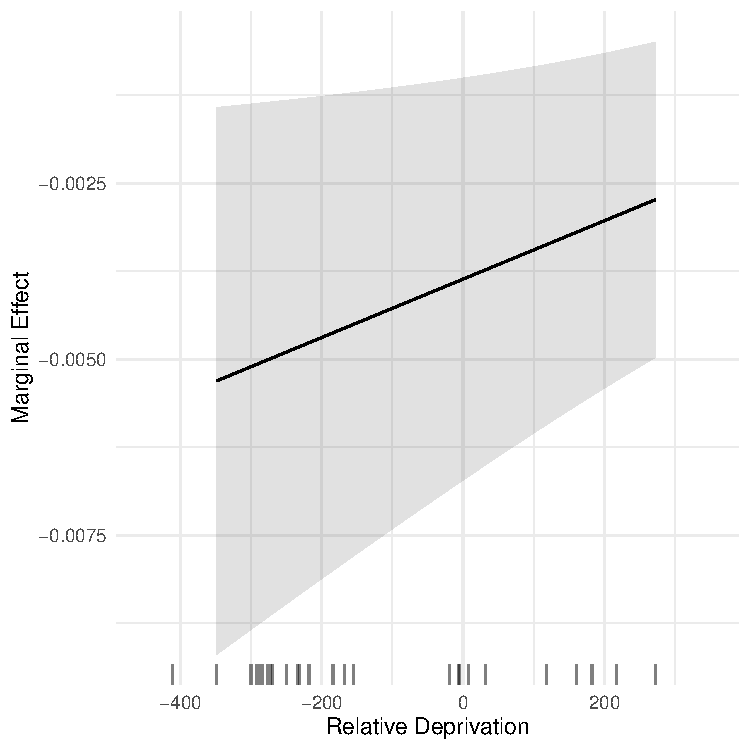
\includegraphics[width=1\textwidth]{figures/me_lpm.pdf}
\end{figure}

\section{Discussion}

In the previous part, it was investigated whether CCTs affect violent unrest in Brazil. Additionally, it was tested whether relative deprivation had a moderating effect on the relationship. In this section, the results will be discussed in light of the literature and theoretical framework. First, it was found that there is a negative and significant relationship between CCTs and violent unrest, which confirms H\textsubscript{1}. This means that the higher the cash transfers in a particular municipality, the lower the probability that the municipality experienced a violent event. The findings thus confirm the results of previous literature \parencite{chiodaSpilloversConditionalCash2016, machadoConditionalCashTransfer2018}.

This speaks to a spillover effect: By reducing the worries of people or immediate poverty and need, people express less violence, both on the individual as well as on the collective level \parencite{litwinConditionalCashTransfer2019, penaCivilConflictConditional2017}. In this paper, it is shown that this link persists over time and across municipalities in Brazil. It is important to take into account that the results do not show a higher level of violence, but rather predict whether any type of violence happens or not, as it has a binary outcome.

Second, relative deprivation was found to positively and significantly moderate the relationship between CCTs and violent unrest in Brazil. In other words, the higher the relative deprivation on a state level, the weaker the relationship between CCTs and violence. As such, H\textsubscript{2} could be confirmed: The negative relationship is weakened. Feeling deprived relative to others makes cash transfers less effective at reducing violence.

In previous literature, it was found that deprivation is tied to an increase in violence \parencite{itskovichEconomicInequalityRelative2025}. As a mechanism, it was expected that it would weaken the relationship. The higher the relative deprivation, proxied by income inequality, the weaker the effects of CCTs on violent unrest. The mechanism is supported by the present paper. This ties back to the theoretical model of Relative Deprivation Theory: In communities where people are more deprived, they develop grievances, which hinders the beneficial effects of CCTs from taking place \parencite{smithRelativeDeprivationTheory2020}. As such, payments are not as effective at reducing violent unrest, as the deprivation amplifies the grievances. Previous research also showed how deprivation is tied to aggression, which could further support the mechanism of this paper, as heightened aggression levels in a population could translate into violence \parencite{greitemeyerImpactPersonalRelative2019}.

Some limitations need to be taken into account. Although the results were significant, the within R\textsuperscript{2} was very low for both regressions, also compared with the adjusted R\textsuperscript{2}. This means that the municipality as well as the time fixed effects were driving the relationship mainly, while the predictor or interaction added barely any explanatory value to the within-municipal variation in violent unrest.. In light of this, the results can only be interpreted with caution. To account for this, future research should use different approaches to see how the model fit could be improved. For example, a Poisson two-way fixed effect model could be a better choice.

Another important limitation is the lack of data on the municipal level for income. As it could not be sourced, the moderator was constructed to work on a state level, which leads to the loss of nuance. Additionally, there are concerns with reverse causality in the baseline model. Municipalities that have higher violence might receive more payments, rather than payments pacifying the municipality. For future research, problems with causality should be addressed.

Furthermore, the models did not take into account differences in the programmes. The relationship might be different depending on whether the data are drawn from the \textit{Bolsa Família}, \textit{Auxílio Brasil}, or \textit{Novo Bolsa Família}. For future research, it is recommended to differentiate on the basis of that. For example, it could be tested how the relationship to violence differs depending on the programme.

For further research, it is also advised to look further into other mechanisms. Given that the within R2 was low, there are other variables which could better explain the relationship between the predictor and outcome. Relative deprivation measures are used as a mediator in other research, which would be interesting to test \parencite{jiangRelativeDeprivationMechanism2020}. Additionally, instead of using two-way fixed effects, a model could be fitted using control variables, such as municipal gross domestic product, unemployment, public spending, and electoral results.

Therefore, it can be said that while the results were significant, it is questionable whether wide conclusions can be drawn from them. While a pattern is certainly discernible, the limitations mentioned pose a significant challenge to the validity of the results. However, they pose initial directions to aid future research in further investigating mechanisms behind the CCT–violence link evidenced by this paper, as well as previous literature discussed. As such, it is a stepping stone towards building better models to understand how payments lead to a reduction in violence.

\section{Conclusion}

In conclusion, the outcomes of redistributive policies on violent unrest in Brazil were investigated in this paper. Specifically, the extent to which the \textit{Bolsa Família} CCTs are associated with lower violent mobilisation was examined. To study the theoretical mechanism of relative deprivation, a moderator was added that reflects the differences in income between a respective state and the national average. As evidenced by the results of the analysis, CCT payments reduce the probability of violent unrest within municipalities. Additionally, the interaction term weakened the suppressive effects, which shows that states with higher deprivation experience fewer benefits from the CCT payments. The low explained variation in the outcome needs to be addressed by future research, as it is a stark limitation of this paper. The contribution, however, remains clear: Deprivation remains an important factor to consider in further investigations on the topic.

\printbibliography

\end{document}
